% !TEX root = ../thesis-example.tex
%
\chapter{Reject Options}
\label{sec:options}

\section{Two Classes}
\label{twoclasses}
To make our way towards optimal rejects for multi class classification, we start of small by looking at a general two class classifier $f$ that divides the space via a decision boundary. 
$$ f: \mathbb{R}^n \to \{1,2\} $$
Let $r$ be a measure of confidence that a point is part of its respective class, e.g. distance to the decision boundary. If $r(\bar{x})$ is large it means that $\bar{x}$ is likely in the class it was assigned to.

\begin{figure}[!htbp]
\centering
\caption{Example of two classes separated by a decision boundary. You can see falsely classified points near the boundary which we would like to reject.}
\label{decBound}
\begin{tikzpicture}
	\node {\svg{\textwidth}{2classDecBoundary}};
	\draw[ultra thick] (0.235,-1.25) -- (0.235,1.6);
\end{tikzpicture}
\end{figure}

\subsection{Reject Strategy}
We look for a threshold $\theta$ that defines for a given point $\bar{x}$ whether it is rejected or not:
$$ r(\bar{x}) < \theta : \bar{x} \  rejected $$

\subsection{Optimal $\theta$}
\label{optimalt}
In order to find an optimal threshold we need to decide how to evaluate it. Optimally only wrongly classified data points are rejected (now referred to as true rejects). But generally there will be rejected, although correctly classified, points (false rejects). 
A given labeled data set $X = \{\bar{x}_1,...,\bar{x}_n\}$ (by $y(\bar{x}) \mapsto \{1,2\}$) is divided into the two sets $L$ and $E$ by applying $f$ as a classifier with:
\begin{align} 
L&=\{\forall \bar{x} \in X \ | \ f(\bar{x}) = y(\bar{x})\} : \text{correctly classified points} \\
E&=\{\forall \bar{x} \in X \ | \ f(\bar{x}) \neq y(\bar{x})\} : \text{incorrectly classified points} 
\end{align}
And by applying our reject strategy with the threshold $\theta$, $X$ is divided into $A$ and $R$ with:
\begin{align} 
A_\theta&=\{\forall \bar{x} \in X \ | \ r(\bar{x}) \geq \theta \} : \text{accepted points} \\
R_\theta&=\{\forall \bar{x} \in X \ | \ r(\bar{x}) < \theta\} : \text{rejected points} 
\end{align}
The set $T$ contains all true rejects and $F$ all false rejects.
\begin{align} 
T_\theta &= R \cap E \\ 
F_\theta &= R \cap L
\end{align}
Naturally we want $|T_\theta|$ to be large and $|F_\theta|$ to be small. Since these two goals often contradict each other, e.g. more true rejects most times bring more false ones (see figure \ref{incTaF}), in general there is no single optimal choice of $\theta$. Still there is a set of values that we consider optimal. As shown above each $\theta$ corresponds to a tuple $(|T_\theta|,|F_\theta|)$. $\theta$ is optimal if
$$ \nexists \theta^{'} : |F_\theta^{'}|\leq|F_\theta|, |T_\theta^{'}|\geq|T_\theta| $$ and at least one inequality holds, thus being Pareto optimal.

\begin{figure}[!htbp]
\centering
\caption{In this example we can see the corresponding true and false rejects if $r(\bar{x})$ is chosen as a threshold for each $\bar{x} \in X$. $r(\bar{x})$ is increasing from the bottom left corner to the upper right. As we can see, the number of false and true rejects are monotonically increasing with a more strict threshold.}
\label{incTaF}
	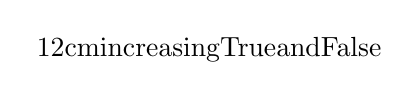
\begin{tikzpicture}
		\node {\svg{12cm}{increasingTrueandFalse}};
	\end{tikzpicture}
\end{figure}

\subsection{Finding $\theta$}
\label{findt}
Now that we know how to evaluate our thresholds we still need to know where to look for them. Obviously $\theta$ needs to be in the range of $r$ so
$$ \Theta := \{\theta \in \mathbb{R} \ | \ \theta < \operatorname*{max}_{\bar{x}} r(\bar{x})\}  $$
is the set of possible thresholds. Because this set is infinitely large we need to reduce the its size (TODO:wording). We recognize that it is sufficient to only consider the discreet set of the values of $r$. So with $\Theta := \{r(\bar{x}) | \forall \bar{x} \in X\}$ we have a feasible set of possible thresholds. It can be refined by looking again at our criteria for an optimal $\theta$. Let 
$$ \bar{r} = (r_1,...,r_n) \ | \ r_i = r(\bar{x}_i) \forall \bar{x}_i \in X, r_j < r_{j+1} \forall j \in \{1,...,n-1\} $$ 
be the vector of thresholds in $\Theta$ sorted by the measure of confidence in ascending order. Consider $\bar{r}(i)$ as threshold with $\bar{x}_i \in E$. We now consider different cases:
\begin{itemize}
	\item $\bar{x}_{i-1} \in E$: $\bar{r}(i-1)$ cannot be a better choice since it would result in one less true reject.
	\item $\bar{x}_{i-1} \in L$: $\bar{r}(i-1)$ is a better threshold since it gives an additional true reject.
	\item $\bar{r}(i+1)$ cannot be a better threshold since it only adds a false reject.
\end{itemize}
In conclusion this means that it is sufficient to consider only points at the beginning of groups of false rejects, giving us
$$ \Theta := \{r(\bar{x}_i) \ | \ \bar{x}_i \in L, \ \bar{x}_{i-1} \in E\} $$
as an easily computed set of thresholds to consider to be optimal (see figures \ref{possibleThresholds} and \ref{paretoFront}.)

\begin{figure}[!htbp]
\centering
\caption{This figure shows the thresholds from before (see figure \ref{incTaF}). The green marked points correspond to threshold we consider optimal.}
\label{paretoFront}
	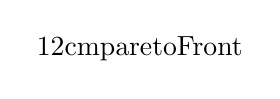
\begin{tikzpicture}
		\node {\svg{12cm}{paretoFront}};
	\end{tikzpicture}
\end{figure}

\begin{figure}[!htbp]
\centering
\caption{This is an example of classified points sorted by a measure of confidence. You can see that $r(\bar{x}_2)$ and $r(\bar{x}_7)$ are the only sensible thresholds. Choosing $r(\bar{x}_8)$ instead of $r(\bar{x}_7)$ would only add a false reject and choosing $r(\bar{x}_6)$ over $r(\bar{x}_7)$ would result in one less true reject.}
\label{possibleThresholds}
\begin{tikzpicture}
	\node[draw=none] at (0.6,1.2) {$r(\bar{x}) \rightarrow$};
	\draw[style=thick] (0,0) rectangle (10,1);
	\draw[fill=white] (0.5,0.5) circle (0.35) node {$\bm{\bar{x}_1}$};
	\draw[fill=myBlue,text=white,draw=myBlue] (1.5,0.5) circle (0.35) node {$\bm{\bar{x}_2}$};
	\draw[fill=myBlue,text=white,draw=myBlue] (2.5,0.5) circle (0.35) node {$\bm{\bar{x}_3}$};
	\draw[fill=white] (3.5,0.5) circle (0.35) node {$\bm{\bar{x}_4}$};
	\draw[fill=white] (4.5,0.5) circle (0.35) node {$\bm{\bar{x}_5}$};
	\draw[fill=white] (5.5,0.5) circle (0.35) node {$\bm{\bar{x}_6}$};
	\draw[fill=myBlue,text=white,draw=myBlue] (6.5,0.5) circle (0.35) node {$\bm{\bar{x}_7}$};
	\draw[fill=myBlue,text=white,draw=myBlue] (7.5,0.5) circle (0.35) node {$\bm{\bar{x}_8}$};
	\draw[fill=myBlue,text=white,draw=myBlue] (8.5,0.5) circle (0.35) node {$\bm{\bar{x}_9}$};
	\draw[fill=white] (9.5,0.5) circle (0.35) node {$\bm{\bar{x}_{10}}$};
	
	\draw[ultra thick] (1,1) -- (1,0) node [label=below:{$\theta_1$}] {};
	\draw[ultra thick] (6,1) -- (6,0) node [label=below:{$\theta_2$}] {};
	
	\draw[fill=white] (0.5,-2) circle (0.35);
		\node[draw=none] at (2.9,-2) {falsely classified points};
	\draw[fill=myBlue,draw=myBlue] (0.5,-3) circle (0.35);
		\node[draw=none] at (3.1,-3) {correctly classified points};
\end{tikzpicture}
\end{figure}


\section{Multi class Classification}
Let us now expand the problem to a classifier for $N$ multiple classes.
By using a one vs all strategy, we get $N$ binary classifiers $f_k$ like in chapter \ref{twoclasses} and an according measure of confidence $r_k$. Points are now classified in the class where confidence is maximal among all classes. This gives us a multi class classifier $f$ with
\begin{align}
 f: \mathbb{R}^n &\to \{1,...,N\} \\
   \bar{x} &\mapsto \operatorname*{arg\,max}_k r_k(\bar{x}) 
\end{align}

\subsection{Global Reject}
To adapt our reject strategy from before, we search for a threshold $\theta$ and reject according to our measures of confidence:
$$ \operatorname*{max}_k r_k(\bar{x}) < \theta \ : \ \bar{x} \ \text{rejected}  $$
We look again to choose $\theta$ so that it meets our requirements for an optimal threshold (see chapter \ref{optimalt}). This strategy comes with the problem that it relies on all measures $r_k$ to be scaled the same way. While there might be a workaround for this, e.g. using probabilities as scale, a global reject is still imprecise when the internal structures of the classes differ a lot(see figure \ref{classStructure}). A reasonable threshold for a class with most points and also most classification errors near the decision plane is probably not well suited for a class with a larger variance in its set of data points. This leads to the idea of having individual thresholds for each class.

\begin{figure}[!htbp]
\centering
\caption{In this two-class classification example one class (blue circles) has few errors near the decision boundary and the other (red triangles) multiple further away. A global reject optimal for the first class would result in a lot of unrejected errors in class 2. Conversely an optimal global reject for class 2 would result in many false rejects in class 1.}
\label{classStructure}
\begin{tikzpicture}
	\node {\svg{\textwidth}{classStructure}};
	\draw[ultra thick] (-0.5,-0.9) -- (-0.5,1.3);
\end{tikzpicture}
\end{figure}

\subsection{Local Reject}
\label{localreject}
To account for differences in class structure each one now has a local reject threshold $\theta_k$. A point is rejected if
$$ r_k(\bar{x}) < \theta_k \ | \ \forall \bar{x} \  \text{where} \ f(\bar{x}) = k $$
This gives us an N-dimensional threshold vector $\bar{\theta} = (\theta_1,...,\theta_N)$. Each $\theta_k$ regulates the reject practice only in their respective class. (TODO: example)

\subsection{Optimal Local Reject}
For each threshold $\theta_k$ the same criteria apply to determine if it is optimal as for a global threshold (see chapter \ref{optimalt}). With the difference that we look at each class individually. So the true and false rejects are now given by
\begin{align} 
T_{\theta_k}^k &= R_{\theta_k}^k \cap E_k \\ 
F_{\theta_k}^k &= R_{\theta_k}^k \cap L_k \\
\forall \theta_k \in \Theta_k &:= \{r_k(\bar{x}_i) \ | \ \bar{x}_i \in L_k, \ \bar{x}_{i-1} \in E_k\}, \ \forall k \in \{1,...N\}
\end{align}
where $R_{\theta_k}^k$ is the amount of rejected points in class $k$ given the threshold $\theta_k$, $E_k$ the set of falsely classified points in class $k$ and $L_k$ the set of correctly classified points in $k$. We conclude that the threshold vector $\bar{\theta}=(\theta_1,...,\theta_N)$ is optimal if each $\theta_k$ is optimal. Conversely an optimal $\theta_k$ is not necessarily a component of an optimal vector $\bar{\theta}$.


\subsection{Computation by Brute Force}
To now find the optimal local reject vectors $\bar{\theta}$ with a brute force approach we need to consider every combination of thresholds in the sets $\Theta_k$. Let
$$ \mathbb{P} = \left\{\bar{\theta} = \left(\theta_1,...,\theta_N\right) \in \Theta_1 \times ... \times \Theta_N \right\} $$
be the set of all choices from the sets of optimal thresholds of each class. Algorithm \ref{bruteForce} describes in pseudo code how to find all optimal $\bar{\theta}$.

\begin{algorithm}[!htbp]
 \KwData{$\mathbb{P}$}
 \KwResult{set of optimal local reject vectors $\Theta_{opt}$}
 initialization\;
 array $opt$ where $opt(n)$ is the maximum number of true rejects with n false ones \;
 array $theta$ where $theta(n)$ is the optimal threshold vector with n false rejects \; 
 \ForEach{$\bar{\theta} \in \mathbb{P}$}{
 	$F :=$ amount of false rejects for $\bar{\theta}$ \;
 	$T :=$ amount of true rejects for $\bar{\theta}$ \;
 	\If{$opt(F)<T$}{
 		$opt(F):=T$ \;
 		$theta(F)=\bar{\theta}$ \;
 	}
 }
 \KwRet{theta}
 \BlankLine \BlankLine
 \caption{Computing optimal local reject options by brute force.}
 \label{bruteForce}
\end{algorithm}

\subsection{Computation by Dynamic Programming}
\label{dp}
Computation by brute force scales exponentially with the number of classes and is therefore not a feasible solution for large data sets with lots of clusters. But our problem is equivalent to a multiple choice knapsack problem (MCKP) where thresholds within a class correspond to items, false rejects correspond to costs, and true rejects correspond to their value (TODO:link). This allows us a faster solution that still maintains optimal results.
Let

$$
opt(n,j,i) = \max_{\bar{\theta}}
\begin{Bmatrix}
	 & \left|F_{\bar{\theta}}\right| \leq  & n \\
  	\left|T_{\bar{\theta}}\right| \ s.t. & \theta_l \in & \Theta_l \forall l < j \\
  	 & \theta_j \in & \left\{\bar{\theta}_j(0),...,\bar{\theta}_j(i)\right\} \\
  	 & \theta_l \in & \bar{\theta}_l(0) \forall l > j
\end{Bmatrix}
$$
with 
\begin{align}
	n &\in \{0,...,|L|\} \\
	j &\in \{1,...,N\} \\
	i &\in \{0,...,\left|\Theta_j\right|-1\} \\
	\bar{\theta}_k &= (\theta_1,...,\theta_n) \ | \ \theta_i \in \Theta_k, \ \theta_j < \theta_{j+1} \forall j \in \{1,...,n-1\} (TODO)
\end{align}
be the maximum number of true rejects with $n$ false rejects while considering all thresholds in classes before class $j$ and the first $i$ thresholds in class $j$. All $\bar{\theta}$ corresponding to $opt(n,N,\left|\Theta_N\right|-1) \forall n<\left|L\right|$ fulfill our criteria for an optimal threshold vector. \\
This results in the Bellmann equation \ref{DP} to efficiently compute $opt$:

\begin{subnumcases}{opt(n,j,i) = \label{DP}}
\text{if} \ n=0 : &$ \ \sum_{k=1}^{N} \left|T_{\bar{\theta}_k(0)}^k\right|$ \label{DPcase1}\\
\text{if} \ n>0\text{,}\ j=0 : &$ \ \sum_{k=1}^{N} \left|T_{\bar{\theta}_k(0)}^k\right|$ \label{DPcase2}\\
\text{if} \ n>0\text{,}\ j>0\text{,}\ i=0 : &$ opt\left(n,j-1,\left|\Theta_{j-1}\right|-1\right)$ \label{DPcase3}\\
\text{if} \ 0<n<\left|F_{\bar{\theta}_j(i)}^j\right|\text{,}\ j>0 :  &$ opt\left(n,j,i-1\right)$ \label{DPcase4}\\
\text{if} \ n \geq \left|F_{\bar{\theta}_j(i)}^j\right|>0\text{,}\ j>0 :  &$ max\Bigg\{opt\left(n,j,i-1\right),$ \notag \\
&$\ opt\left(n-\left|F_{\bar{\theta}_j(i)}^j\right|,j-1,\left|\bar{\theta}_{j-1}\right|-1\right)+$ \notag\\
&$\ \left|T_{\bar{\theta}_j(i)}^j\right|-\left|T_{\bar{\theta}_j(0)}^j\right|\Bigg\}$ \label{DPcase5}
\end{subnumcases} 



Each case is explained as follows:
\begin{itemize}
\item Case \ref{DPcase1}: $n=0$ means that no false rejects are allowed so the first threshold (index 0) in each class is chosen. The resulting amount of true rejects is summed up over all classes.
\item Case \ref{DPcase2}: $j=0$ means that no class is under consideration for a threshold. So we stay with the first threshold in each class (see above). 
\item Case \ref{DPcase3}: $i=0$ means that no threshold is under consideration in class $j$. So we look in the previous cell with the strictest threshold possible.
\item Case \ref{DPcase4}: The chosen threshold $i$ in class $j$ exceeds the allowed amount of false rejects, so the next less strict threshold is considered.
\item Case \ref{DPcase5}: Here the $i$th threshold in $j$ is a possible threshold but it is not clear whether it is optimal. We consider both cases. If it is not the optimal threshold, we take the next less strict one. If it is optimal, we continue our search in the previous class but with $|F_{\bar{\theta}_j(i)}^j|$ less allowed false rejects in consequence to choosing this threshold. The other consequence is that this threshold results in a number of gained true rejects compared to the least strict threshold and this gain is added.
\end{itemize}

This Bellmann equation can be computed by dynamic programming (see algorithm TODO). We use three nested loops over $n$, $j$ and $i$. This results in a processing time of $\mathbb{O}(|L| \cdot N \cdot \max_k \left|\Theta_k\right|)$. 
Note that this equal in effort to the previous method in (TODO:ref to reject paper) but that the worst case is far less likely to occur here since it would mean that there are no clusters of classification errors. Every grouping of falsely classified points means less computation time than the previous method.

\subsection{Greedy Computation}
\label{greedyAlg}
Computation by dynamic programming gives us an optimal local reject option, but it still might be unfeasible in some cases since it "scales quadratically with the number of data" (TODO: quote reject paper). Hence we are looking for a greedy approximation with linear running time. For this approach we define
\begin{align}
 	\bigtriangleup T_{\bar{\theta}_k(j)}^k = T_{\bar{\theta}_k(j)}^k-T_{\bar{\theta}_k(j-1)}^k \\
	\bigtriangleup F_{\bar{\theta}_k(j)}^k = F_{\bar{\theta}_k(j)}^k-F_{\bar{\theta}_k(j-1)}^k
\end{align}
as the amount of true and false rejects gained by a threshold compared to its predecessor and
$$ g = \bigtriangleup T_{\bar{\theta}_k}^k - \bigtriangleup F_{\bar{\theta}_k}^k $$
as the local gain. The greedy approach lies within choosing the thresholds with the best local gain. Initially all thresholds are set to the most tolerant in each class. Looking at the next strict one in each class we pick the one with the highest local gain until the strictest possible thresholds are reached. The pair of true and false rejects $\left(T_{\bar{\theta}_k}^k,F_{\bar{\theta}_k}^k\right)$ is saved in each step if it is an improvement to an existing solutions. Algorithm \ref{greedy} details this procedure in pseudo code. 

\begin{algorithm}[!htbp]
 \KwData{sets of thresholds $\Theta_k$}
 \KwResult{set of optimal local reject vectors $\Theta_{opt}$}
 initialization\;
 array $opt$ where $opt(n)$ is the maximum number of true rejects with n false ones \;
 array $theta$ where $theta(n)$ is the optimal threshold vector with n false rejects \; 
 $\bar{\theta} = \left\{\bar{\theta}_0(0),...,\bar{\theta}_N(0)\right\}$ \; 
 $F :=$ amount of false rejects for $\bar{\theta}$ \;
 $T :=$ amount of true rejects for $\bar{\theta}$ \;
 \While{a more strict threshold in at least one class exists}{
 	\ForEach{$\theta_k(j) \in \bar{\theta}$}{
 		\eIf{$\exists \theta_{i}(j+1)$}{
 			$g(k) = \bigtriangleup T_{\bar{\theta}_k(j+1)}^k - \bigtriangleup F_{\bar{\theta}_k(j+1)}^k$ \;
 		}{
 			$g(k) = -\infty$ \;
 		}	
 	}
 	$\hat{k}=\operatorname*{arg\,max}_k g(k)$ \;
 	set threshold $\theta_{\hat{k}}(j)$ in $\bar{\theta}$ to $\theta_{\hat{k}}(j+1)$ \;
 	$T = T +  \bigtriangleup T_{\bar{\theta}_{\hat{k}}(j+1)}^{\hat{k}}$ \;
 	$F = F +  \bigtriangleup F_{\bar{\theta}_{\hat{k}}(j+1)}^{\hat{k}}$ \;
 	\If{$opt(F)<T$}{
 	 	$opt(F):=T$ \;
 	 	$theta(F)=\bar{\theta}$ \;
 	}
 }
 \KwRet{theta}
 \BlankLine \BlankLine
 \caption{Computing optimal local reject options by greedy evaluation.}
 \label{greedy}
\end{algorithm}

\section{Evaluation}
In this chapter we evaluate the described methods. We try to confirm the optimality of the dynamic programming method by comparing its result to the brute force algorithm. Furthermore we want to find out how close the greedy approach is to being optimal.

\subsection{Data Sets}
For our evaluation we use randomly generated data sets. Using a normal distribution we get random samples of points divided into two classes, above and below $0$. We now introduce further normal distributions at random locations to get cluster of falsely classified points (see figure \ref{dataset}).

\begin{figure}[!htbp]
\centering
\caption{Example of a small generated data set with one cluster of falsely classified points in each class.}
\label{dataset}
\begin{tikzpicture}
	\node {\svg{\textwidth}{rndDataSet}};
	\begin{axis}[hide axis,
	  no markers, domain=0:10, samples=200,
	  axis lines*=left, xlabel=$x$, ylabel=$y$,
	  every axis y label/.style={at=(current axis.above origin),anchor=south},
	  every axis x label/.style={at=(current axis.right of origin),anchor=west},
	  height=2.5cm, width=6cm,
	  xtick={4,6.5}, ytick=\empty,
	  enlargelimits=false, clip=false, axis on top,
	  grid = major,
	  at={(-400,-260)}
	  ]
	  \addplot [thick,myBlue!50!black] {gauss(1.35,0.3)};
	  \addplot [thick,myBlue!50!black] {gauss(8.95,0.3)};
	\end{axis}
	
\end{tikzpicture}
\end{figure}

\subsection{Methods}
In regards to our definition of an optimal threshold (see chapter \ref{optimalt}) we use the true and false rejects of each threshold considered to be optimal by the respective method. To further see the behavior of the reject options we introduce a measure of quality of the classification in a second evaluation method. (TODO: ref to arc paper).


\subsection{DP vs Brute Force}
\label{DPvsBF}
Since there is no formal proof that the Bellman equation (see chapter \ref{dp}) finds every optimal reject option we compare its result to the outcome of the brute force method. We can see in figure \ref{dpEvaPareto} that the results match for nine different generated data sets. Although this is, of course, no proof we conclude for now that the dynamic programming algorithm finds optimal thresholds.

\begin{figure}[!htbp]
\centering
\caption{This figure shows the true and false rejects for the thresholds considered optimal by dynamic programming(red crosses) and by brute force(red circles) on different randomly generated data sets. We can see that the results coincide in each case. }
\label{dpEvaPareto}
\begin{tikzpicture}
	\node {\svg{\textwidth}{dpComp}};
\end{tikzpicture}
\end{figure}

\subsection{DP vs Greedy}
\label{DPvsGR}
We now compare the results of the greedy strategy (see chapter \ref{greedyAlg}) to the optimum. If the results are nearly accurate it is a feasible solution for big data sets since its running time is linear. We can observe in figure \ref{greedyEvaPareto} that the results of the greedy computation are mostly close to being optimal or even optimal and that far outliers are rare and not extreme (TODO:wording). Using our second evaluation method (see figure \ref{greedyEvaARC}) we can observe that the greedy reject options lead to a very similar quality of classification as the ideal ones (TODO: again wording).

\begin{figure}[!htbp]
\centering
\caption{Comparison of the thresholds computed greedily (red crosses) and the optimal ones computed by dynamic programming (green circles) on randomly generated data sets. We can see that the greedy strategy is close to optimal and sometimes falls off slightly if a lot of points are rejected.}
\label{greedyEvaPareto}
\begin{tikzpicture}
	\node {\svg{\textwidth}{greedyComp}};
\end{tikzpicture}
\end{figure}


\begin{figure}[!htbp]
\centering
\caption{ARCs for data sets classified with optimal rejects (green curve) and with greedy rejects (red dashed curve).}
\label{greedyEvaARC}
\begin{tikzpicture}
	\node {\svg{\textwidth}{greedyARC}};
\end{tikzpicture}
\end{figure}
